\documentclass[a4paper, 12pt]{report}

%% Pour des marges plus équitables.
\usepackage[margin=2cm]{geometry}
%% Pour la langue des titres et sous-titres.
\usepackage[francais]{babel}
%% Pour de belles images.
\usepackage{graphicx}
%% Pour la police de caractères.
\usepackage{fontspec}
%% Pour les liens externes.
\usepackage[hidelinks]{hyperref}
%% Pour pouvoir écrire du code.
\usepackage{minted}
%% Arrière plan des blocs de code.
\definecolor{bg}{rgb}{0.95,0.95,0.95}

\setmainfont{Sansation Light}

\begin{document}
\begin{titlepage}
	\vspace*{\fill}
	\begin{center}
		{\Huge Thésaurus, l'analyse}\\
		\vspace{\fill}
		Franck Petitdemange \\
		Nordine El Hassouni \\
		Issam Amal \\
		Cyril Monmouton \\
		Marouane Denguiri \\
		Mohamed Amine Zahir \\
		Abdelhamid Belarbi
	\end{center}
	\vspace*{\fill}
	\center{\today}
\end{titlepage}

\tableofcontents

\begin{chapter}{Genèse}
	\begin{section}{Le groupe et le sujet}
		Le groupe est constitué des sept personnes nommées sur la page de garde et le responsable du projet est Abdelhamid Belarbi
		\footnote{Élu démocratiquement à 71,42 \% des voix.}.\\
		Nous avons choisi de traiter le thème de l’\emph{astronomie} au sens large du terme. Nous inclurons donc des termes tels que \emph{Comète},
		\emph{Galaxie}, \emph{Étoile} ou bien \emph{Voie Lactée}.
	\end{section}
	
	\begin{section}{Définitions}
	\label{aspic}
		Internet regorge de définitions de thésaurus et des notions qui s’y rapportent (voir \cite{Wikipedia}, \cite{Inpes}, \cite{Bdsp} et \cite{Unesco}).
		Toutefois, beaucoup d’entre elles sont peu claires, très vagues voire obscures. En tant que concepteurs d’une application, nous nous devions de réunir les
		meilleures définitions, les clarifier et les spécifier sans ambiguïté.\\
		
		
		
		\noindent
		Nous utiliserons les définitions suivantes.
		\begin{subsection}{Définitions globales}
			\begin{description}
				\item[\emph{Terme} :] mot ou combinaison de mots significatifs.
				\item[\emph{Descripteur} :] terme choisi pour caractériser les informations, aide à l'indexage et la recherche (= terme préférentiel ou vedette).
				\item[\emph{Non-descripteur} :] terme non accepté à l'indexation, il peut s'agir de synonyme, abréviation ou variante orthographique d'un descripteur
				(= terme non préférentiel ou
				synonyme).
				\item[\emph{Microthésaurus} :] ensemble de descripteurs reliés au même concept. Noté \emph{MT}.
				\item[\emph{Thésaurus} :] ensemble de micro-thésaurus.
			\end{description}
		\end{subsection}
		
		\begin{subsection}{Pour les relations entre termes}
			\label{glouglou}
			\begin{description}
				\item[\emph{EP (Employé Pour)} :] relation entre un descripteur et le (ou les) non-descripteur qu'il référence.
				\item[\emph{EM (Employer)} :] relation entre un non-descripteur et son descripteur (symétrique de la relation précédente).
				\item[\emph{TA (Terme Associé)} :] relation entre des descripteurs appartenants à des micro-thésaurus différents, mais entre lesquels peuvent exister des
				proximités sémantiques.
				\item[\emph{TS (Terme Spécifique)} :] relation entre un descripteur plus général et un (ou plusieurs) descripteur plus spécifique.
				\item[\emph{TG (Terme Général)} :] relation entre un descripteur plus spécifique et un descripteur plus général (symétrique de la relation précédente).
			\end{description}
		\end{subsection}
		
		\begin{subsection}{Pour les modes d'indexation}
			\begin{description}
				\item[\emph{Liste alphabétique structurée} :] Les descripteurs sont affichés par ordre alphabétique avec leur relations sémantiques.
				\item[\emph{Liste par micro-thésaurus} :] Les descripteurs sont affichés hiérarchiquement, du plus général au plus spécifique.
				\item[\emph{Liste alphabétique permutée} :] Les termes sont affichés selon les notions dans lesquelles ils apparaissent.
			\end{description}
		\end{subsection}
	\end{section}
\end{chapter}

\begin{chapter}{Analyse}
	\begin{section}{Spécifications}
		Les fonctionnalités que nous voulons faire figurer dans l'application sont les suivantes :
		\begin{itemize}
			\item Recherche par mot clé sur l'ensemble des descripteurs;
			\item Affichage du thésaurus indexé des trois manières possibles;
			\item Interface d'administration permettant d'ajouter et de manipuler des termes.
		\end{itemize}
		
		Ces différentes fonctionnalités sont décrites plus en détail dans le diagramme suivant.
	\end{section}
	\begin{section}{Diagramme Use-Case}\label{re}
		\begin{figure}[h]
			\label{sucresale}
			\begin{center}
				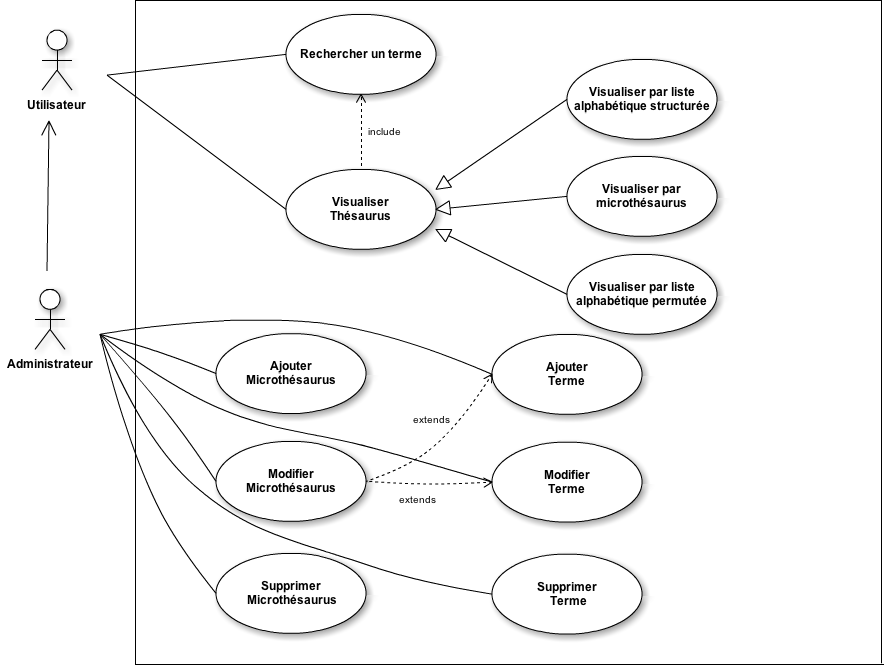
\includegraphics[width=12cm]{Use-Case.png}
				\caption{Le diagramme des cas d'utilisation}
			\end{center}
		\end{figure}~\\
		
		\begin{subsection}{Analyse textuelle}
			Quelques précisions s'imposent quant au diagramme précédent.\\
			\begin{itemize}
				\item L'utilisateur est un simple visiteur anonyme.
				\item La recherche s'effectue en spécifiant un mot-clé et un mode d'affichage (d'indexation).
				\item Visualiser un thésaurus revient soit à le voir en entier avec tout les termes de la base,
					soit un seul micro-thésaurus, soit un seul terme avec tous les termes auxquels il est lié.
				\item Lorsque l'administrateur ajoute ou modifie un terme, il peut spécifer le micro-thésaurus auquel il appartient d'où les flèches \emph{<<extends>>}.
			\end{itemize}
		\end{subsection}
	\end{section}
\end{chapter}

\begin{chapter}{Conception}
\label{tournevis}
	\begin{section}{Diagramme des classes}
		\begin{figure}[h]
			\label{classeur}
			\begin{center}
				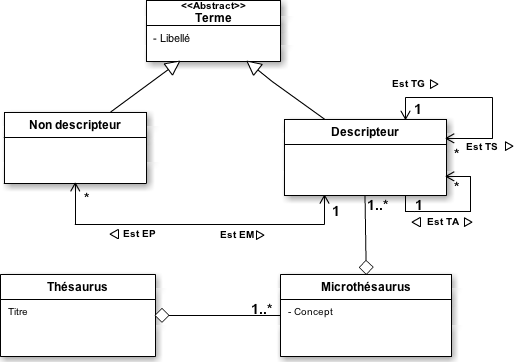
\includegraphics[width=13cm]{Classes.png}
				\caption{Le diagramme des classes}
			\end{center}
		\end{figure}~\\
		
		Le diagramme parle de lui-même. Toutes les définitions données dans la section \ref{aspic} sont appliquées, d'où l'utilité de la démarche de clarification effectuée.\\
	\end{section}
\newpage
	\begin{section}{Base de données}
	Le schéma objet-relationnel est directement inspiré du diagramme des classes. Il se présente de la manière suivante (code ODL).\\~\\
	\begin{minted}[bgcolor=bg]{java}
interface Terme {
	attribute string libelle;
}

class Descripteur:Terme {
	relationship list(NonDescripteur) EP      // Employé pour
	             inverse NonDescripteur::EM;
	relationship list(Descripteur) TA         // Termes associés
	             inverse Descripteur::TA;
	relationship list(Descripteur) TS         // Termes spécifiques
	             inverse Descripteur::TG;
	relationship Descripteur TG               // Terme général
	             inverse Descripteur TS;
	relationship Microthesaurus MT
	             inverse Microthesaurus::concept;
}

class NonDescripteur:Terme {
	relationship Descripteur EM;              // Employer
}

class Microthesaurus {
	attribute string concept;
	relationship list(Descripteur) descripteurs
	             inverse Descripteur::MT
}

class Thesaurus {
	attribute string titre;
	relationship list(Microthesaurus) microthesaurus;
}
	\end{minted}

	Concernant la classe \emph{Thesaurus}, il est à noter qu'elle est
	inutile puisque nous ne traitons qu'un seul thésaurus. Mais par souci de clarté et par respect des définitions et du sujet 
	nous la mettons quand même.\\


	Pour ce qui est des autres classes la transformation est triviale, chaque lien d'association est traduit par la relation
	correspondante. Nous avons choisi d'utiliser des \emph{list} pour représenter les données multiples. Les relations inter-objets seront
	explicitées grâce au type \emph{REF}.\\

	Remarquez de plus que les opérations des objets ne sont pas représentées ici car il ne s'agit globalement que d'accesseurs.\\
	\end{section}

	\begin{section}{Et les vues}
		Il est assez judicieux de penser à créer des vues pour représenter les différents modes d'indexation afin notamment d'optimiser le temps
		de travail du serveur. \\
		On peut penser par exemple à une vue \emph{listeAlphabetiquePermutee} qui se présenterait de la sorte :\\
		\begin{minted}[bgcolor=bg]{java}
view listeAlphabetiquePermutee {
	libelle string;
	TG string;               // Le libellé du terme général
	TA list(string);         // Les libellés des termes associés
	EP list(string);         // Les libellés des termes employés
}
		\end{minted}

		En étudiant cette vue d'assez près on se rend compte qu'elle possède à peu de chose près la même structure que la table \emph{Descripteur}.
		C'est sur cette table (et uniquement celle là) qu'il faut effectuer une requête pour construire cette vue. C'est donc une sorte de redondance
		des données.\\

		Pour mettre à jour les vues il faut implémenter différents triggers qui se déclencheront à la mise à jour des tables concernées (ici \emph{Descripteur}).
		Ces ajoutent des traitements du SGBD  pas forcément utiles.

		Le mieux pour représenter les 3 modes est d'effectuer 
		une requête par mode. Ainsi nous tirons parti de la notation pointée de l'objet-relaionnel 
		qui nous permet d'écrire \mint{java}|self.tg.libelle| plutôt que de faire une jointure comme en relationnel.\\

		Ce sont toutes ces raisons qui nous dispensent d'écrire des vues dans notre base objet-relationnel.

	\end{section}
\end{chapter}

\begin{chapter}{Réalisation}
	\begin{section}{Choix des outils}
	L'essor des technologies du web ces dernières années à fait que nous avions une large palette d'outils à notre disposition. Nous avons fait le choix,
	lors d'une réunion de groupe, d'utiliser les outils suivants :
	\begin{itemize}
		\item Pour le back-end, le langage PHP avec un projet organisé selon le modèle MVC.
		\item La base de données sera gérée par Oracle Express utilisant le langage SQL.
		\item Pour le front-end, une interface Html/Css tout ce qu'il y a de plus classique.
	\end{itemize}~\\

	En plus des outils déjà cités nous avons décidé d'utiliser \emph{Smarty}, un générateur de template pour PHP qui simplifie grandement l'affichage des vues.\\
	Les versions du projet furent gérées par \emph{Git}. D'ailleurs voici le lien vers le dépôt :

	\begin{center} \url{https://github.com/AbdelBa/Thesaurus}\end{center}

	Nous avons aussi discuté via Google Groupes pour organiser les réunions, poser les questions publiques et synchroniser notre travail.
	\end{section}

	\begin{section}{Répartition des tâches}
		La taille du groupe nous permet de travailler sur chaque partie du projet simultanément, nous avons donc divisé le groupe en sous-équipes,
		chacune chargée d'une partie de la besogne.
		\begin{enumerate}
			\item{Équipe SQL} : Issam et Abdelhamid
			\item{Équipe PHP} : Franck, Marwan, Cyril et Mohamed
			\item{Équipe Graphisme} : Nordine
		\end{enumerate}

		L'équipe \emph{SQL} fut chargée de l'implémentation de la base de données. C'est à dire la création des types objets, des tables ainsi 
		que tout élément nécessaire au bon fonctionnement de l'application.\\
		L'équipe PHP devait programmer les solutions à intégrer au modèle MVC. Ce qui signifie faire les classes, les scripts de connexion à la 
		base de données, la logique metier...\\
		L'équipe singleton de Nordine était chargée de faire une interface graphique simple et sobre et de paufiner le travail de l'équipe PHP
		sur les vues.
	\end{section}

	\begin{section}{Details techniques}
		Jusqu'à maintenant tout se passait bien, une immense plaine verdoyante s'étendait de toutes parts à perte de vue et la brise légère faisait
		onduler nos cheveux de manière quasi-imperceptible.\\ Mais lorsqu'il s'est agi de programmer, commencèrent à émerger ça et là divers tourments
		que voici énumérés.

		\begin{subsection}{L'affaire Oracle Express}
			Oracle propose sur son site une version de son célèbre SGBD dénommée Oracle Express. À notre grand désarroi cette version n'est disponible
			que pour Windows x32 ou Linux x64 et c'est tout.\\
			Autant dire que les deux membres du groupe possesseurs d'un ordinateur Apple étaient hors course, eux qui fanfaronnaient si souvent avec leur
			machine en aluminium ne pouvaient même pas faire fonctionner Oracle Express dans une machine virtuelle.\\
			Mais l'affaire fut vite réglée lorsque ils prirent la décision de venir travailler à l'université.\\

			Bien sûr il y avait un outil en ligne fourni par Oracle même, Apex (voir [\ref{cloche}]), mais la base de données qui est procurée au développeur n'est
			disponible qu'au sein même d'Apex sans possibilité de connexion externe.
		\end{subsection}

		\begin{subsection}{SQL}
			Le lecteur attentif aura remarqué que dans le chapitre \ref{tournevis}, les relations entre les différentes classes sont drôlement
			entremêlées (voyez la classe \emph{Descripteur}). SQL n'offre pas la possibilité de faire des références en avant,
			ce qui pose un problème lorsque deux types dépendent l'un de l'autre. La solution réside dans ce qui est appelé dans la documentation les types
			incomplets. Voici comment nous avons mis en oeuvre cette solution (voir le fichier \emph{src/modeles/sql/types.sql}) : \\~\\
			\begin{minted}[bgcolor=bg]{sql}
-- Créations de types incomplets pour les références en arrière.
CREATE OR REPLACE TYPE NonDescripteur_t UNDER Terme_t (); /
CREATE OR REPLACE TYPE Descripteur_t UNDER Terme_t (); /

-- Une table imbriquées pour stocker une liste de non descripteurs.
CREATE OR REPLACE TYPE ListeNonDescripteurs_t AS 
    TABLE OF REF NonDescripteur_t; /

-- Type Descripteur_t
ALTER TYPE Descripteur_t ADD ATTRIBUTE (
    EP ListeNonDescripteurs_t
)CASCADE;

-- Type NonDescripteur_t
ALTER TYPE NonDescripteur_t ADD ATTRIBUTE (
    EM REF Descripteur_t
)CASCADE;
			\end{minted}
		\end{subsection}

		\begin{subsection}{PDO}	
			Nous avons d'abord un peu hésité à utiliser le driver PDO pour oracle de PHP car il est écrit dans la documentation [\ref{claque}], 
			dans un grand cadre rouge que \og Ce module est EXPERIMENTAL. Cela signifie que le comportement de ces fonctions, leurs noms et, concrètement, TOUT ce qui est documenté ici peut changer dans un futur proche, SANS PREAVIS ! \fg \\
			Comme le projet ne devait pas durer trop longtemps et que l'ancien driver (OCI8) n'était pas fait en objet nous avons quand même utilisé PDO.\\

			Les problèmes rencontrés avec de module ne se situaient pas là mais plutôt au niveau de la configuration des 
			différents acteurs, à savoir PHP (via le fichier \emph{.ini}) et le serveur Apache. Il faut savoir que sous
			Windows, le driver PHP ne fonctionne qu'avec un serveur 32 bits, étrange...
		\end{subsection}
	\end{section}
\end{chapter}

%% Sitographie
\renewcommand\bibname{Webographie}%% Changement du titre de bibliographie en webographie.
\begin{thebibliography}{2}
	\bibitem{Wikipedia}
	L'encyclopédie que l'on ne présente plus, utile pour les définitions.\\
	\emph{Adresse} : \url{fr.wikipedia.org}
	~\\
	\bibitem{Inpes}
	Un thésaurus très bien fait qui est présenté dans les trois modes d'indexation.\\
	\emph{Alphabétique structuré} : \url{www.inpes.sante.fr/30000/pdf/thesaurus/thes\_01.pdf}\\
	\emph{Microthésaurus} : \url{www.inpes.sante.fr/30000/pdf/thesaurus/thes\_02.pdf}\\
	\emph{Alphabétique permuté} : \url{www.inpes.sante.fr/30000/pdf/thesaurus/thes\_03.pdf}
	~\\
	\bibitem{Bdsp}
	Le (très) gros thésaurus de la Banque de données en Santé Publique, très instructif.\\
	\emph{Adresse} : \url{asp.bdsp.ehesp.fr/Thesaurus/}
	~\\
	\bibitem{Unesco}
	Le thésaurus de l'Unesco, une autre aide précieuse pour bien comprendre les principes.\\
	\emph{Adresse} : \url{databases.unesco.org/thesfr/}
	~\\
	\bibitem{Oracle SQL reference}
	La documentation Oracle officielle pour faire du SQL dans les normes.\\
	\emph{Adresse} : \url{docs.oracle.com/cd/E11882_01/server.112/e26088/toc.htm}
	~\\
	\bibitem{PDO doc}\label{claque}
	La documentation de PHP PDO.\\
	\emph{Adresse} : \url{fr2.php.net/manual/fr/ref.pdo-oci.php}
	~\\
	\bibitem{Oracle Apex}\label{cloche}
	Le service web qui fournit une base de données consultable via le navigateur.\\
	\emph{Adresse} : \url{apex.oracle.com}
\end{thebibliography}

\end{document}
